


\chapter{Future Work SORT}


\section{SORT Rough Notes}

try consistent approaches to \gls{internal rate of return}


what does a speculative over investment.  in housing  do? - hollowed out store front

who carries what risks- banks vs individuals

subdivision and density

multiple cities,
linear cities

differential skills and wages,
work from home

details of typologies, transportation networks, etc

- make it available as a part for other models, use other models in this model


% % TEMP - here are some other notes we may want to reference or bring in. [[non individualistic modeling of agents]] [[generalizability in agent vs classical econ models]]



From model chapter ``Transaction costs on the sale are omitted. They are actually large. We can easily add a term to  Equation~\ref{eqn:maximum-bid} to examine the effect of transaction costs on the distribution of wealth.''

Amplified effects by extensions
Two city experiments
Different incomes  - inequality
Urban density



model development (experiments and extensions)
interventions
theoretical development
% The urban production sector pays a wage premium $w$
%This is a convenient simplification, not a necessary feature of the model. 

The rental value of land shapes the city spatially.  

\section{Experiments with this model}
Lots of simple extensions e.g. 2 cities with immigration, differentiated labour, products, market power, neighbourhood effects (see extensions map/typology), we focus on those elements central to seeing the structure of the resilience dynamics of the wealth/housing effect. Consider adding density, to look at how it interacts with agglomeration effects. (integrating with transportation effects is neat)


- why people hold onto baby boomer homes
- what happens with suburbanization
- speculative agent cycle- 
- pernicious cycle - lean into investment, rentals, lowered interest and increased supply actually amplify the problem
- pumps wealth out on the way up and on the way down


Potential interventions and systems shifts.. oasis cities..





\subsection{Initial state}
Basic experiments has all homes owner occupied to start. Other initial tenure mixtures are easily modelled. WHY WE MIGHT WANT TO

The basic model can be initialized by matching the number of properties to the size of the population. 

In the simplest version, firms concentrate at the city centre. Workers are spread over space and pay transportation costs to commute.

The size of the city is determined by population and lot size. Income and transportation costs will interact with lot size. 

\subsection{Parameter values}

\subsection{Analysis methods}
mapping of regimes

\subsubsection{Net benefit}
Net benefit may be economically interesting later.

If an agent owns a home, after maintenance and taxes the \textbf{net benefit B} in each period is 
\[B= \omega-cd +(a-ab)\phi +\mathbb{A} - \tau P^{assesssed}\]
Capitalizing this we get a measure of the value of net benefits.

If the assessed price is a fraction, say $\kappa$, of the warranted price
\[B^{capitalized}=\frac{\omega-cd +(a-ab)\phi + \mathbb{A}}{(1- \tau\kappa)r}\]


\subsection{Data}
incorporation of local data more carefully

\section{Extensions to the model}
The simple circular city can be extended to to produce other forms, including polycentric cities and hierarchies of cities at the cost of additional computational complexity. The simple case we examine will allows us to focus on the general, and neglected, distributional features of this class of models.

\subsection{Financialization vs expansion of the housing stock}

Financialization is not expansion of the housing stock, it is transfer of ownership. It is a process orthogonal to development.

% - it can lead to efforts to extract more rents by displacing people to invest in a shift in built form.
There are a number of potential links with the development process.

\begin{figure}
\begin{center}
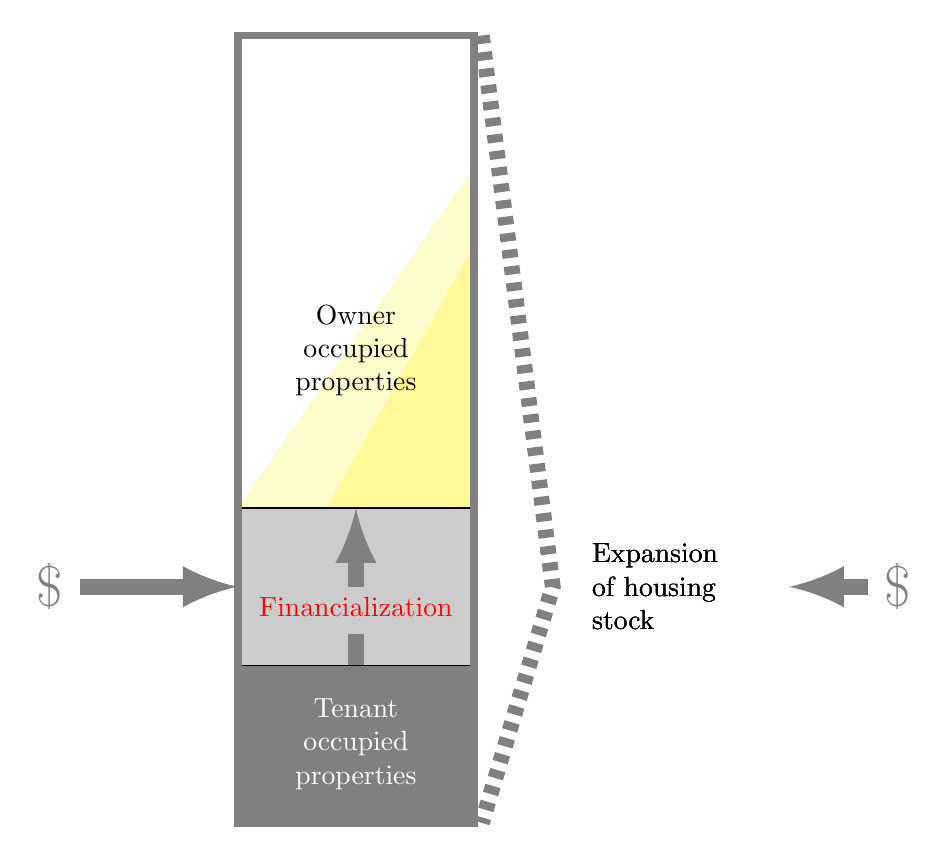
\begin{tikzpicture}{scale=.5}
\draw [fill=yellow!20] (0,4)--(3,4)--(3,8.33); --cycle;% MORTGAGE %Calculation. 80\%owner, so  8 above the tenant line. 2/3*8=5.333. 5.333+2=

\draw [fill=yellow!40] (0,2)--(3,2)--(3,7.33); --cycle;% MORTGAGE %Calculation. 80\%owner, so  8 above the tenant line. 2/3*8=5.333. 5.333+2=
\draw [fill=gray!40,opacity=1] (0,0) rectangle (3,4); %fiancialization   
\draw [fill=gray] (0,0) rectangle (3,2); %TENANT

\draw[line width= 1mm, black!50] (0,0) rectangle (3,10);

\node at (1.5,6)
    [text width=2.4cm, align=center]
    {\baselineskip=20pt Owner occupied properties};
%\node at (2,3.3) [text width=2.4cm]  {\baselineskip=20pt Mortgaged};
\node at (1.5,1)
    [text width=2.4cm, align=center, white]
    {\baselineskip=20pt Tenant occupied properties};

%\draw [gray,line width=2mm](1.5,2)--(1.5,2.4) node[above, red]{Financialization}; 
\draw [gray,line width=2mm](1.5,2)--(1.5,2.4) node[above, red]{Financialization}; 
\draw [gray,-latex, line width=2mm](1.5,3)--(1.5,4);
%\draw [gray,line width=2mm,-latex](3,3)--(4,3);
\node at (5.5,3)[text width=2cm]{Expansion of housing stock}; 
\draw [gray, dashed,line width=2mm,](3.1,10)--(4,3)--(3.1,0);

\draw [gray,line width=2mm,-latex](-2,3)node[left]{\huge$\$$}--(0,3); \node at (5.5,3)[text width=2cm]{Expansion of housing stock}; 

\draw [gray,line width=2mm,-latex](8,3)node[right]{\huge$\$$}--(7,3); 
\node at (5.5,3)[text width=2cm]{Expansion of housing stock}; 
\end{tikzpicture}
\end{center}
\caption{Financialization expands investor ownership, but does not in expand the housing stock. Yellow represents privately owned homes for which ownership is partially held by mortgage lenders.}
\label{fig-financialization-expansion}
\end{figure}


\subsection{Lags and adjustment processes}
The details of the adjustment process and the system lags are selected primarily for convenience in simulations. Real-time lags are important and complex, we explore some sensitivity results, but can explore more. 

We model a fairly short lag although in reality lags are long and variable. 

\subsection{Labour adjustment costs}

in the agent model, employees are simply laid off and seek work, so there is unemployment, but there are not \glspl{labour adjustment cost} for firms.

\subsection{Agglomeration effects, and returns to scale}
The case where there are increasing returns at the city level introduces interesting dynamics, explored in appendix CITE % 'furthur discussion' appendix.

We incorporate agglomeration effects using a Cobb Douglas formulation. This allows us to focus on the results of agglomeration in the urban system, rather than specifying the system of firms that transmit the effect. 
There are a number of other ways to study the aglomeration process in more or less explicit ways.

MOVE TO PARAMETER VALUE DISCUSSION?
The strength of the agglomeration is given by $\gamma$, thus for $\gamma=0$ there are not agglomeration effects. APPENDIX?
By definition, with one person, the agglomeration effect has no influence, $\Lambda(1)=1$,  as in the \gls{Cobb-Douglas}, and empirical urban scaling results tell us that agglomeration increases with population, following a power law distribution, so we know %$\die
FIX EQN ERROR die ${\Lambda}{n}>0$. 
%%%%%%%%%. ***WHY
If $\beta=1-\alpha$, this is a \gls{constant returns to scale} production function. Without agglomeration effects, $T(n)=1$,  Then  \textbf{$\mathbf{L(n) = T(n) n}$}  WHAT IS T, WHAT IS THIS TELLING US?
Without agglomeration effects, $\Lambda(n)=1$,  Then  \textbf{$\mathbf{L(n) = T(n) n}$} 


\subsection{Returns to scale and firm under-investment}
Each firm has \gls{decreasing returns to scale}, which means each new worker increases output by less than the previous worker did.
RETURNS TO FIRM CAN BE DECLINING WHILE RETURNS TO CITY INCREASING, THEN FIRM UNDER INVESTS
explore this in the model, see Equation~\ref{eqn-prod1}.

\begin{equation}
Y=K_i^{\alpha }(\Lambda(n)n_i)^{\beta }.
% \label{eqn-prod1}
\end{equation}

MOVE DISCUSSION HERE FOR NOW

\subsection{Heterogeneous agents}
In the simplest model, the central place pays a uniform wage premium, $w$ to all employees, who have identical preferences and transportation costs. 
The wage $w$ is an attribute of individual residents.  
It is straightforward to vary i and to vary preferences. 

relax assumptions and look at how the interaction between the production of social wealth in cities interacts with housing and the extraction of rent to drive patterns in a richer model with heterogenous agents interacting over space and time. 

- wages, skill sets

\subsection{Forward looking agents}
There are reasons to expect the results obtained with  forward-looking agents to differ substantially from those obtained with a model featuring myopic agents.\footnote{For example, Lecca et al. *** \cite{LOST-Lecca-et-al-2013}  used a stylized computational macroeconomic model applicable to a regional context to demonstrate that the assumption of myopic vs forward-looking agents yields differences in the dynamics generated by a shock perturbing the initial steady state, even though the alternative paths lead to the same long-run equilibrium.} 

\subsection{Rental bidding process}
 "Just as with prices, there is an economically \gls{warranted rent} which may differ from the \gls{market rent}. Individuals make their investment decisions on their own expectations rents. the bidding process on rental properties is abstracted in the base model. Instead of modelling the process explicitly, we make the assumption that the warranted rent is the market rent, $\mathcal{R}_W = \mathcal{R}_M$." .. could implement

\subsection{Amenity}
Notation for amenity.
There may be a band surrounding the city or persons who do not commute but enjoy urban consumption amenities. 
based on location etc

\subsection{Preferences}
A utility function/algorithm specifies agents preferences over the attributes that matter. - algorithmic continuous. lexicographic- any traits. 

\subsection{Unemployment and labour adjustment costs}
There is no unemployment. there are no labour adjustment costs for firms. ***INTERESTING TO THINK ABOUT  
when people would stop working with

 falls to subsistence wage -
 too much rent, I guess they leave, they can always move somewhere

\subsection{Insurance, risk, and mortgage backing}

Uncertainty is a key variable.

The effects of policy are large. For example in Canada, backing mortgages is the largest fiscal investment at the national level \cite{nemtinFinancializationHousingSocial2021}.

- risks, bubbles, collapse

Individual sensitivity to uncertainty

\subsection{Moving costs}
     If there are moving costs, people can be trapped in a bad situation, incurring debt, and it can still be not worthwhile to move

\subsection{Mobility}
We could look at mobility in a more sophisticated way..
Agents enter the urban market two ways. If wages rise, agents just outside the city may become commuters. This increases population. 

When homeowners in the city retire they sell their home and move to the country. This allows them  to enjoy the capital value of their home.  They either sell their home or rent it to a new occupant. 

When  tenants in the city retire they would move to the country to enjoy lower rents. This has no effect on population. It is simplest, therefore to treat tenants as permanent residents unless we want the tenant's retirement to trigger an event like a rent increase or a decision by the owner to sell the property.

\subsection{Transportation costs}
Wage and transportation cost determine the radius of the circular city, which determines the size of the labour force which affects urban productivity. The cost of travel is therefore an important variable in the development of urban productivity. 

the transportation cost/distance relationship appears to be non-linear in many cases. While the linear model connects with the established literature, we likely want to explore the implications of more empirically grounded curve (e.g. \cite{bertaudSpatialDistributionPopulation2003}).

\subsection{Multiple firms and production structure}
The scaling result at the level of the city allows us to incorporate the effect of agglomeration in a standard \gls{circular city} model in a simple way. 

We could also explicitly model labour markets and competing firms. 

Explicitly modelling labour markets with multiple firms is a natural way to specify the model more completely, see Appendix~\ref{appendix-future-work},  but it would require introducing many ancillary assumptions and selecting among alternative models of agglomeration, when when we want to focus on distributional and growth-affecting features of the system.

For simplicity, assume firms produce a variety of perfectly substitutable commodities which are exported and locally consumed at a fixed price in a large market. 
***  Increasing product variety may produce a consumption agglomeration economies as in \cite{fujitaSpatialEconomyCities1999}.

\subsection{Market power and interchangeable goods - local markets etc}
MAKE A FOOTNOTE ON MARKET POWER AND INTERCHANGIBLE GOODS??
No externalities imperfect information etc.. ensure efficiency but aren't needed, all you need is price taking for individuals to only pay attention to their own costs and their own benefits. 

\gls{externalities}, \gls{imperfect information}, \gls{monopsony}, \gls{duopoly}, \gls{monopoly}

competitive markets many sellers, many buyers, monopoly single seller, monopsony - single buyer, intermediate cases - monopolistic competition - with some market power but not complete - duopoly- some inefficiency depending on the behavioural model because in the duopoly case they may be able to take advantage of the behaviour of buyers.

Start with perfect competition, then introduce monopolistic competition is most likely.. but it's more difficult to handle. e.g. with brand names, people have some preference for some feature of your particular good so you can price it higher even though you may loose some marginal people. Firms compete on brand name and reputation, not the pure cost effect.

In the spatial economy, goods are deferentially interchangeable. Put them on a line and firms pick a place along they line. Firms are in competition but are competing on a line-.. spatial model moved over to characteristic space..---looking at this would involve overlaying another space - the characteristic space on the physical space. .. There are also local places with local grocery stores. Polycentric stores have effectively monopolistic competition in real space. - like a named cafe downtown has the same.

\subsection{Sectors}
..


\subsection{Incomes}
In the model receive the\gls{urban wage}, which is the subsistence wage plus the urban wage premium $\psi + w$.

They may get different incomes because of firm, sector or individual increases, or particularities of the 
hiring/negotiation/wadge adjustment process, path dependency, stochasticity, etc. 
All of these factors could be explored formally in the model. %ref{rockefeller}


POOR STRUCTURALLY DISADVANTAGED HOWEVER RICH WE GET
these are averages-- some are structurally below average so some are always behind simply because of the structure of the rents claimed.. that's built in FUTURE WORK- DIFFERENT INCOMES GETS YOU THAT. 



\subsection{Hiring process and unemployment} \label{section-rockefeller}
 In our model, non-urban landowners are those who live too far from the urban job center to justify commuting.  Agents join the urban market by adding their names to the firm's list of job applicants when the rent on the marginal unit of land exceeds the transportation cost. 

adjustment speeds..
 
i(did extended modelling in the Rockefeller social innovation lab)- barriers of employment for young people seeking work
- prison records, transportation, family responsibility, bias, educational attainment, expectations of success, neighbourhood factors etc.
Could explore that kind of structure in this model

\subsection{Demographics}
Could build a population model suited to particualr data sets %\ref{section-rockefeller}

\subsection{Skills and individual productivity}
The basic model consideres a non-differentiated workforce. We can add particular skills.
Some agents can be more productive than one another

Agents may move to cities to assemble networks (model as networks)
and learn specialized skills

It can evolve over time so agents can productively over pay to  
-- getting debt/resources at key stages in a persons development to aquire property and skills is important to \gls{wealth trajectories}


\subsection{Sources of agglomeration effects}
Some of the empirically wage difference comes from the dense resources  - location of cities in good places, public investment- libraries - institutions, the network effects
some from the ability of those close to the center to simply claim a larger share of resources
some 
Some of the agglomeration wage may come from people with resources and skills disproportionately choosing cities for their amenity effect. 

We can explore different drivers in the model.


\subsection{TO METHODOLOGY: Rural market and other cities}

 To simplify analysis, we assume that land outside of the residential limit is costless, following th common practice of assuming a fixed price for agricultural land \cite{GET_fixed-price-ag-land}. 

The model is constructed so that there is neither land rent nor capitalist exploitation in the rural economy. 
This special case allows us to examine the distribution of the social surplus generated by agglomeration economies and the effect of financialization.

We could explore this

\section{Interventions: Policy and Agent Strategies}
Extended appropriately, this basic model could be used for planning.

detailed models of interventions typologies of interventions e.g. local currencies, decaying currencies, 

\subsubsection{Teaching}
could use for teaching a sequence for illustration could follow to introduce x ideas - see above. - rent, space, finance treated separately, - tool to think about their relation

productivity centered urban and spatial policy

connects with growth, economic development in real places work

\subsection{Zoning}
zoning - layers interact

\subsection{Taxes}
property taxes reduce the net locational value that flows to an owner but provides services and wages that make the city attractive. 

(create a regime where particular groups have an advantage)

Localized tax advantages can move a share of financilized investment into private consolidation of land.
including structure of taxes for investment properties, institutional investors, individuals, etc.


\subsection{Property transaction costs}
Transaction costs on property sales are omitted. Add a parameter or variable. 
%on sales are omitted. Add a parameter or variable.
The usual form  would be a fixed cost  plus a percentage of the sale price.




\subsection{Housing quality, size, subdivision}
Residents  purchase or rent equal quantities of land at differing locations %$l$ 
for identical housing.  DOWN

? More generally, if we were to introduce variations in lot size and housing types  we would want the integral of the worker density function. In our ABM version  of the model we simply count the workers within the commuter shed.

\subsection{Development and Improvements} \label{sec-extensions-conversion}
% \subsection{Redevelopment and housing characacteristics}
The supply of land at any distance from the center is inelastic. 
Its value comes from proximity to the productive urban centre, not from the value of improvements made to the property.

*** Without density, the labour supply increases with the square of the wage.  other forms..

- We have an empirical curve - gives density- simply build in

- We can .. Model a subdivision process-- urban SIM, a collaborator on the missing middle grant. - model of pro-forma and typoloties/ policies makes it possible to follow..

Some nonlinearities e.g. Some may buy land seeking to develop property in the future and let it become run down. 

We could add improvements
 or consolidation, subdivision, and development. 

% Reference sections on development which is different, and the contribution of amenity % Because supply is fixed for urban land, and the landowner has a monopoly claim on rents, the rents that can be depend on wages and amenity rather than the cost of improvements made to the property.
% The source of rents is the free gifts of nature, the coming together of people to create value in cities, and the concentration of public amenity in cities. 

% ADDD SOMETHING FROM THIS REF?  Capozza et al \cite{capozzaFundamentalsLandPrices1989} show that land price has four additive components: the value of agricultural land rent, the cost of conversion, the value of accessibility, and the value of expected future rent increases. The first two can be treated as a constant.\footnote{Section~\ref{sec-extensions-conversion}, in Appendix~\ref{appendix-future-work}, discusses the potential for more detailed modelling of the land assembly and development process.} The third and fourth two are the focus of this thesis. The value of accessibility in our model is determined by the urban wage premium, which rests on the productivity of the city. Expected future rent increases are driven by increases in the value of accessibility, which is to say, the rising productivity of the city. Productivity rises in our model due to pure agglomeration effects. Our concern is with what happens to the city and its people when financial capital captures the growing value generated by the agglomeration process.  



% Allow redevelopment and construction and allow for decisions about scale, type and location A modelling device that plays a major role is our use of the \gls{urban wage premium}, the difference between a rural and an urban wage driven by positive \gls{agglomeration effect}s on productivity in the city. It cannot be competed away because transportation costs limit access to the productive centre. The wage premium is a partial measure of the agglomeration effect. It generates the \gls{rent premium} on urban land. In this thesis we want to call attention to the distribution of that rent premium.

% To simplify the analysis, we assume that we can partition actual wages between the wage premium,  and all other expenses. The wage premium  is available for consumption, accumulation or to be spent on transportation. Tranportation cost is determined by location, the remainder is available for consumption or appropriation by landowners. We assume both urban and non-urban populations  receive a \gls{subsistence wage} which covers  the cost of buildings, food and other living costs and a base cost of land. This analytical device appears in classical models (Malthus, Ricardo, Marx) as a subsistence wage. In most urban models it is described as the cost of agricultural land, or more precisely,  as the opportunity cost of urban land at the margin. We simply extended the technique to combine the opportunity cost of urban labour and land, allowing us to focus on urban agglomeration rents. 


% There are advantages and disadvantages to this technique. The motivating advantage is that it lets us isolate the social surplus generate by agglomeration. One disadvantage is that it suppresses many issues that are of interest in other contexts -- such as choice of home size and quality. In the computational model it is easy to allow for different building types and more complex housing choice, but in this section we simply  want to make the logic of our model as clear as possible. We foresee adding layers to the computational model that incorporate redevelopment and construction and allow for decisions about scale, type and location. 

% Another disadvantage of technique in the analytical version is that it does not allow us to make visible speculation on  the value of  buildings as opposed to the locational value. It is a problem that is dealt with in the computation model, but we believe the added complexity will not add clarity here. Research (see \cite{mcdonaldWilliamAlonsoRichard2007}) has shown  that the core \gls{Alonzo model}, driven entirely by locational rents,  is robust to many extension of this sort. 





\subsection{Overlapping generations}
In our model individuals have a working life, then retire. If they own homes they sell and move to the countryside where housing is cheaper. They are replaced by new entrants from the countryside. New entrants may become buyers or tenants. This is a variant of the \gls{overlapping generations}  model in which savings are passed on to the next generation. In our case, access to individual  homes is passed on as agents retire and move away. While the model has multiple generations, it is not a `dynastic' model in which the generations are linked by family ties and inheritance matters in individual decision-making. We rely on this simple version because the core issues for us are the effect of financialization on city productivity, on whether the city continues to provide opportunity for newcomers and those without the benefit of generational wealth, and on the emergence of classes driven by the financial system. Introducing a richer family structure would complicate the model but add little to understanding  our main issue. 








\section{TO  METHODOLOGY?: Distribution}% not the right word
ABMs can be run multiple times to produce distributions of expected outcomes, which makes them valuable in planning exercises. They also do not require that we use a representative agent to make them tractable. Our model is intended to be elaborated  for such use. 

extensions
what it is
why it would be great to model
why it doesn't matter for our core results



\section{Theory - how to pay for innovation?}

Leaving land out, however, creates a problem in  the neoclassical growth theories we will examine below. John B. Davis \cite{davisRicardoTheoryProfit1993} noted that ``Questions arise, however, when one turns to exchange between a sector paying rent and one not.'' 
Under the assumption of perfectly competitive goods and factors markets as well as marginal productivity pricing of capital and labour, neoclassical growth requires technical change to be generated outside the model because there are no resources left to innovate if both factors of production are paid their marginal product.\footnote{This follows from Euler's theorem: if, for a given level of technology $\bar A$ output Y is produced according to a \textbf{constant returns to scale} and twice continuously differentiable function of capital and labour $F(K, L, \bar A)$, Euler's theorem implies that $F_K K + F_L L=Y$, where $F_i$ is the marginal product of factor $i$. Payments to  capital and labour take up the entire national product and no resources are left to finance the production of technology-improving innovations. are paid their marginal product.} 
If, however, land is reintroduced, as it must be in an urban model, there must be rents and there is therefore a surplus available for innovation.
\footnote{An alternative and common approach is to assume imperfect competition, which may be based on increasing returns to scale, in which case firms with market power may achieve a surplus. ``Although seldom modeled outside the monopolistic competition framework, market incompleteness and imperfect competition are central to the new growth theories'' (Gilles Duranton, Growth and imperfect competition on factor markets: Increasing returns and distribution, European Economic Review, 44-2, 2000, 255-280), Similarly, Sjak Smulders and Theo van de Klundert conclude that ``Growth is higher in a more concentrated market provided that market power of firms is not too high,'' (Imperfect competition, concentration and growth with firm-specific R \& D, European Economic Review, 39-1, 1995,139-160).}













\subsection{Implications}
\subsubsection{Agglomeration driven under-investment}

\section{Extensions of the Alonso model}

The Alonzo model has been used to illustrate a wide range of urban issues. Incorporating these extensions, we can explore relatively fine-grained effects of financialization. The examples that follow  illustrate   ways the model can be extended and suggest further hypotheses that we  would like to test using our model.